
\subsection{Deviation From Put-Call Parity}
The put-call parity relations derived from \textcite{stoll1969relationship} is a classical option pricing concepts in finance. It characterized the relationship that must exist between European put and call options with the identical underlying asset, expiration and strike prices. The equation must hold for European options given on no-dividends paying underlying in a perfect market. 
\begin{equation}
C-P = S - PV(K)
\end{equation}
Where C and P represent call prices and put prices, and S is Stock price. With same maturity and exercise price K, the arbitrage opportunity would exist if the equation does not hold. The \textcite{black1973pricing} formula satisfies the put-call parity for an assumed value of the volatility parameter $\sigma$, therefore, 
\begin{equation}
C^{BS}(\sigma ) + PV(K) = P^{BS}(\sigma ) + S
\end{equation}
where $C^{BS}(\sigma )$ and $P^{BS}(\sigma )$ indicate Black-Scholes call and put prices, respectively. 
\\
Combine the above equation, we can derive the equation
\begin{equation}
C^{BS}(\sigma ) - C = P^{BS}(\sigma ) - P
\end{equation}
which implies that the implied volatility of call option and put option should be the same if all equation holds. 
\begin{equation}
IV^{call} = IV^{put}
\end{equation}
Of course, the equation may not hold once the option is American-style. However, our primary studies, SPX option, is European style. Therefore, we do not need to consider the dividend payment or early exercise case in our further research. 

Clearly, the larger the implied volatilities, the higher the call (put) options prices claim. Following \textcite{amin2004index}, we refer to the difference between call and put implied volatilities as the call-put implied volatility spreads (CPIV). It is suggested that a positive (negative) CPIV could be viewed as a bullish (bearish) signal regarding the underlying stock. 

The aggregate Intraday CPIV are construced as following steps: 
\begin{enumerate}
\item  We first divided a single day into 14 of 5-minutes intervals. Each interval contains the tick data from 2.5 minutes ahead and behind the clock. For example, the 9 a.m. interval, we collect valid data from 08:47:30 to 09:32:30 to represent this interval. As for open (close) interval, we choose to accumulate the full 5 minutes data behind (ahead)\footnote{We collect the whole transaction data in 5 minutes for trade data. However, the size of quote data is extremely unbalanced in different intervals, we restricted 1000 to 2000 quotes as maximum for call and put in collecting quote data.}

\item Similar to \textcite{xing2010does}, in each interval, we eliminate an option from the sample if its time to expiration is less than 10 days or more than a year, if its open interest is negative, if its moneyness\footnote{Moneyness is defined as the ratio of the strike price to the stock price.} is smaller than 0.9 or more than 1.1. Furthermore, the option quotes must not violate basic no-arbitrage relations.

\item Then, in each time interval, there must be several valid option pairs with identical maturity (T) and exercise price (K). For each option pair, we choose only one pair to be the representative. For quote data, we average the best bid ($\beta ^{\ast }$) and best offer ($\alpha ^{\ast }$) as the chosen call (put) option price. On the contrary, for trade data, we seize the specific transaction data which is closet to the centering time.  

\item After collecting several time interval valid option pairs. we calculated the CPIV by applying, 
 \begin{equation} \label{eq: withoutadj}
CPIV_{t} = IV_{t}^{call} - IV_{t}^{put} = \sum_{j = 1}^{N_{t}}\theta _{j,t}(IV_{j,t}^{call} - IV_{j,t}^{put})
 \end{equation}
 
$CPIV_{t}$ denotes the implied volatility spread on interval $t$; $IV_{j,t}$ describe the B-S implied volatility for $j^{th}$ option pair in time $t$; $\theta_{j,t}$ are the weight for $j^{th}$ option pair in time $t$, there are $N_{t}$ valid pairs of options on interval $t$. 

Follow by \textcite{holowczak2013aggregating}, the aggregation of option information could be adjusted by the level of moneyness and maturity. 
 \begin{equation} \label{eq: withadj}
CPIV_{t} = IV_{t}^{call} - IV_{t}^{put} = \sum_{j = 1}^{N_{t}}w_{j,t}(IV_{j,t}^{call} - IV_{j,t}^{put})
 \end{equation}

The equation is identical except for the weights term. Ceteris paribus. $w_{j,t}$ equals to $exp(-(m_{j}^{2})/2 -(M_{j} - 1)^{2}) * \theta_{j}$ where $m_{j}^{2}$ measures the moneyness and the $M_{j}$ evaluates the maturity of option contract $j$. To be more specific, $m_{j} =  (\frac{K_{j}}{S_{j}} - 1)$ and $K_{j}$ represents the exercise price and $S_{i}$ acts for the underlying price of option $j$; $M_{j} =  max(1, T_{j}*12) $ and $T_{j}$ represents the maturity of option $j$ in month unit. 


\end{enumerate}


\subsection{Data}
In our analysis, the primary quote and trade intraday data for SPX option originates from CBOE MDR. The sample period studied is from January 2007 to December 2017. The options data includes trade date, trade time, expiration date, put-call code, exercise price, maturities, bid price, ask price, underlying price. The daily price of S\& P 500 index is obtained from Bloomberg. The zero-coupon bond (ZCB) rate represent risk-free rate in B-S formula are collected from WRDS with different duration. The size of the sample data is about 1-TB around and the data amount is about 1 billion. After we exclude the tick data fall outside the 14 of 5-minute intervals, it remains about 40 million. Furthermore, we follow the approach from \textcite{ofek2004limited} to exclude the invalid option pairs. Finally, we have 1,692,542 valid volatility spreads for SPX option from January 2007 to December 2017. 

Following the prior studies \textcite{bollerslev2009expected}, several macro-economic variables are suggested to be crucial and informative with regard to future returns. Specifically, we collect data of the default spread (between Moody's BAA and AAA corporate bond spreads), the term spread (between the 10-year T-Bond and 3-month T-bill yields) \footnote{The daily data are collected from the public website of the Federal Reserve Bank of St. Louis.} as control variables in our regression analysis. The set of macro-economics controls used in regressions changes as the measurement window of the expected market returns changes. 

In our study, the amount of intraday CPIV should be 38,668 (14 Intervals multiply 2,762 Days). However, most of the option quote data are short date contract (less than 10 days) in the middle of the month so that we have multiple values that are not able to calculate by our approach. Meanwhile, our research also winsorized the outliers of intraday CPIV on 1\% at the front and end. The amount of final valid interval CPIV of quote data is 27,554, as for trade data is 36,959.


\autoref{table:stats_of_CPIV} presents the descriptive statistics of intraday CPIV. In panel A, we demonstrate the descriptive statistics on CPIV of intervals. The mean (median) CPIV vary from -2.45 \% to -3.65 \% (-3.32 \% to -3.72\%), indicating that, on average, S\&P 500 index put option has about three percent higher implied volatility than index call option during our sample period. In fact, the results are similar to \textcite{atilgan2015implied}, they put forth the observation that on average there are nine percent higher during their sample period. In the index market, the implied volatility to moneyness graph mostly shows a reverse skew, which prior studies \parencite{zhang2008implied} claimed it volatility smirk. Our observations also express this phenomenon. In addition, in panel A, we could tell that the CPIV of open interval (08:30) is completely different from other interval CPIV. The mean of $CPIV_{0830}$ is about 1\% higher than other intervals, and the standard deviation of $CPIV_{0830}$ is 0.4\% higher than others. Furthermore, the amount of positive CPIV is way larger than other intervals. We suggest during the open interval, numerous news and trading information flow in and cause the open-interval CPIV more volatile. Furthermore, the call options are more likely to be relatively expensive than put options in the first interval. We suggest that if investors exposure to good news before the market open, they prefer to reflect on option price in the first 5-minutes.  

In panel B, we test the population mean among the intervals CPIV. 
\begin{equation}
H0: \mu _{i} = \mu _{j}
%H1: \mu _{i} \neq  \mu _{j}
\end{equation}
The p-values of pairs are shown in corresponding rows and columns. From the results, we declare that the population means of $CPIV_{0830}$ are significantly different from other intervals, so does the close interval CPIV. In other words, we claim that the population means of mid-interval CPIV are not significantly different from other mid intervals. The mid intervals may gather similar information. 






%\subsection{Figure}
%\autoref{fig:Network} stock trading volume, and stock returns data are taken from CRSP for the construction of control measures.
%
%\begin{figure}[h]
%\centering
%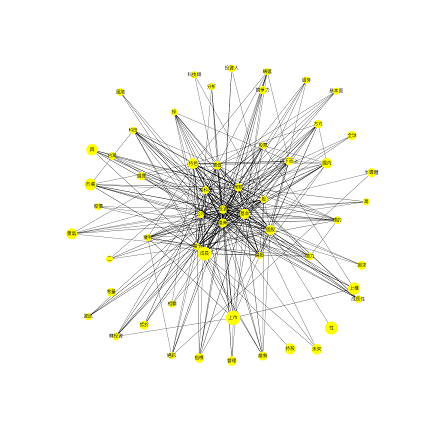
\includegraphics[scale=1.0]{network1}
%\caption{Network ot words}
%\label{fig:Network}
%\end{figure}


\subsection{Empirical Methodology}
Our research divided into two parts. The first part we analysis certain option pair characteristics that cause the deviation of put-call parity. The second part we discuss the relationship between CPIV and index returns in different aspects and frequencies. 

Firstly, we regress CPIV on options characteristics like moneyness, time non-synchronization, maturity, and controlling on intervals effect. The CPIV term and moneyness term are in absolute form because we care about the level of deviations in put-call parity rather than the direction of deviations. 

 \begin{equation}\label{eq:char}
 \footnotesize
\left | CPIV _{i} \right| = \alpha  + \beta _{1}TimeDiff_{i} + \beta _{2}\left |Moneyness_{i} \right | + \beta _{3}Maturity_{i} +  \beta _{j} \sum_{j=1}^{13}IntDummy_{j} +\varepsilon _{i}
 \end{equation}

$TimeDiff_{i}$ represents time non-synchronization in option pair $i$. $Moneyness_{i}$ stands for the level of divergence between the underlying price and the excersie price of option pair $i$. $Maturity_{i}$ symbolizes the maturity date in option pair $i$. As for $IntDummy_{j} $, we control the intervals effect where $j$ denote as each interval, for instance, $IntDummy_{1}$ stands for 09:00. All the t statistics are \citeauthor{newey1986simple} statistics adjusted. 

Secondly, we regress contemporaneous index returns, one day ahead index returns, halh-hours ahead index returns on CPIV and other macroeconomic variables respectively. 
 \begin{equation}  \label{eq:contem}
SPX\_Return_{t} = \alpha + \beta _{1}CPIV_{t} + \beta _{2}DEF_{t} + \beta _{3}TERM_{t} + \varepsilon _{t}
 \end{equation}

In above equation, $SPX\_Return_{t}$ elucidates the SPX index returns in day $t$, where $CPIV_{t}$ could be any interval CPIV within day $t$. $DEF_{t}$ explicates the change in the difference between the yields on BAA- and AAA-rated corporate bonds in day $t$, and $TERM_{t}$ expounds the difference between the yields on the 10-year Treasury bond and one-month Treasury bill in day t. All the t statistics are \citeauthor{newey1986simple} statistics adjusted. 

\begin{equation} \label{eq:1dayahead}
SPX\_Return_{t+1} = \alpha + \beta _{1}CPIV_{t} + \beta _{2}DEF_{t} + \beta _{3}TERM_{t} + \varepsilon _{t}
\end{equation}

In equation (9), the only term we change is $SPX\_Return_{t+1}$. We now regress a day forward returns on dependent variables rather than contemporaneous index returns. 

\begin{equation}
\small
Intra\_Return_{t, k} = \alpha + \beta _{1}CPIV_{t} + \beta _{2}DEF_{t} + \beta _{3}TERM_{t} + \varepsilon _{t},    
\forall k = 1, 2...13-n  
\end{equation}

In this part, we would like to discuss the predictability in intraday index returns, where $Intra\_Return_{t, k}$ means $k$ of half-hour ahead cumulative returns. For example, when we'd like to do research on the intraday returns to $CPIV_{0830}$, $k = 1$ means the cumulative returns from 08:30 to 09:00, and  $k = 2$ means the cumulative returns from 08:30 to 09:30, and so on and so forth. $n$ represents the $n^{th}$ interval CPIV.



